%%%%%%%%%%%%%%%%%%%%%%%%%%%%%%%%%%%%%%%%%%%%%%%%
% E.Pinault-Bigeard - e.pinault-bigeard@upsti.fr
% http://s2i.pinault-bigeard.com
% CC BY-NC-SA 2.0 FR - http://creativecommons.org/licenses/by-nc-sa/2.0/fr/
%%%%%%%%%%%%%%%%%%%%%%%%%%%%%%%%%%%%%%%%%%%%%%%%
\documentclass[11pt, multicol]{article}
%%%%%%%%%%%%%%%%%%%%%%%%%%%%%%%%%%%%%%%%%%%%%%%%
% Package UPSTI_Document
%%%%%%%%%%%%%%%%%%%%%%%%%%%%%%%%%%%%%%%%%%%%%%%%
%%%%%%%%%%%%%%%%%%%%%%%%%%%%%%%%%%%%%%%%%%%%%%%%
% Package UPSTI_Document
%%%%%%%%%%%%%%%%%%%%%%%%%%%%%%%%%%%%%%%%%%%%%%%%
\usepackage{subcaption}
\usepackage[usenames, svgnames, dvipsnames]{xcolor}
\usepackage{UPSTI_Document}
\usepackage{pgfplots}
\usepackage{import}
\definecolor{darkspringgreen}{rgb}{0.09, 0.45, 0.27}

\newcommandx*{\dessinRepereFigGeo}[5][1=\vx{},2=\vy{},3=\vz{},4=,5=0]
	{
		\draw [->,very thick] (0,0) -- (1,0) ;
		\draw [->,very thick] (0,0) -- (0,1) ;
    \fill[white] (0,0) circle (0.13);
    \draw [->,very thick] (0,0) circle (0.13);
    \ifnumequal{#5}{0} {% z vers nous
      \fill[black] (0,0) circle (0.03);
      \draw [->,thick] (0,0) circle (0.04);
    }{% z vers la feuille
  		\begin{scope} [rotate=45]
  			\draw [-,thick] (0,-0.12) -- (0,0.12) ;
  			\draw [-,thick] (-0.12,0) -- (0.12,0) ;
  		\end{scope}
    }
		\draw [anchor=north west] (1.1,0) node {${#1}$};
		\draw [anchor=south west] (0,1.1) node {${#2}$};
		\draw [anchor=north east] (-0.1,0) node {${#3}$};
		\draw [anchor=north west] (-0.1,-0.1) node {${#4}$};
	}

	\usepackage{array}
	\newcolumntype{L}[1]{>{\raggedright\let\newline\\\arraybackslash\hspace{0pt}}m{#1}}
	\newcolumntype{C}[1]{>{\centering\let\newline\\\arraybackslash\hspace{0pt}}m{#1}}
	\newcolumntype{R}[1]{>{\raggedleft\let\newline\\\arraybackslash\hspace{0pt}}m{#1}}

	\usepackage{pifont}% http://ctan.org/pkg/pifont
\newcommand{\cmark}{\color{green}\ding{51}}%
\newcommand{\xmark}{\color{red}\ding{55}}%
\newcommand{\fmark}{\ding{229}}%
\newcommand{\itemc}{\item[\cmark]}%
\newcommand{\itemx}{\item[\xmark]}%
\newcommand{\itemf}{\item[\fmark]}%

\usepackage{multirow}
%---------------------------------%
% Paramètres du package
%---------------------------------%

% Version du document (pour la compilation)
% 1: Document prof
% 2: Document élève
% 3: Document à publier
\newcommand{\UPSTIidVersionDocument}{2}


% Classe
% 1: PTSI				6: PSI*			11: TSI2		16: Spé
% 2: PT	(par défaut)	7: MPSI			12: ATS
% 3: PT*				8: MP			13: PC
% 4: PCSI				9: MP*			14: PC*
% 5: PSI				10: TSI1		15: Sup
%\newcommand{\UPSTIidClasse}{2}



% Matière
% 1: S2I (par défaut)    2: IPT     3: TIPE
% 6: Vie au lycée
\newcommand{\UPSTIvariante}{5}
\newcommand{\UPSTIidMatiere}{0}
\newcommand{\UPSTIintituleMatiere}{Automatique}
\newcommand{\UPSTIsigleMatiere}{Autom}
% Type de document
% 0: Custom*				7: Fiche Métho de			14: Document Réponses
% 1: Cours (par défaut)		8: Fiche Synthèse    		15: Programme de colle
% 2: TD     				9: Formulaire
% 3: TP						10: Memo
% 4: Colle					11: Dossier Technique
% 5: DS						12: Dossier Ressource
% 6: DM						13: Concours Blanc
% * Si on met la valeur 0, il faut décommenter la ligne suivante:
%\newcommand{\UPSTItypeDocument}{Custom}
\newcommand{\UPSTIidTypeDocument}{1}

% Titre dans l'en-tête


% Titre dans l'en-tête

\newcommand{\UPSTIvariante}{5}

\newcommand{\UPSTItitreEnTete}{Automatisme industriel}
%\newcommand{\UPSTItitreEnTetePages}{}
\newcommand{\UPSTIsousTitreEnTete}{Introduction aux API}


% Titre
%\newcommand{\UPSTItitrePreambule}{Automatisme industriel}
\newcommand{\UPSTItitre}{La programmation d'un Automate Industriel}

% Durée de l'activité (pour DS, DM et TP)
\newcommand{\UPSTIduree}{3h30}

% Note de bas de première page
%\newcommand{\UPSTInoteBasDePremierePage}{Geoffrey Vaquette}
% Numéro (ajoute " n°1" après DS ou DM)
\newcommand{\UPSTInumero}{2}

% Numéro chapitre
%\newcommand{\UPSTInumeroChapitre}{1}

% En-tête customisé
%\newcommand{\UPSTIenTetePrincipalCustom}{UPSTIenTetePrincipalCustom}

% Message sous le titre
%\newcommand{\UPSTImessage}{Message sous le titre}


% Référence au programme
%\newcommand{\UPSTIprogramme}{\EPBComp \EPBCompP{B1-02}, \EPBCompP{B2-49}, \EPBCompS{B2-50}, \EPBCompS{B2-51}, \EPBCompP{C1-07}, \EPBCompP{C1-08}}

% Si l'auteur n'est pas l'auteur par défaut
%\renewcommand{\UPSTIauteur}{WWOOOOOOWW}

% Si le document est réalisé au nom de l'équipe
%\newcommand{\UPSTIdocumentCollegial}{1}

% Source
\newcommand{\UPSTIsource}{G. Vaquette, A. Juton, J. Deprez, J. Maillefert}

% Version du document
\newcommand{\UPSTInumeroVersion}{1}

%-----------------------------------------------
\UPSTIcompileVars		% "Compile" les variables
%%%%%%%%%%%%%%%%%%%%%%%%%%%%%%%%%%%%%%%%%%%%%%%%


%%%%%%%%%%%%%%%%%%%%%%%%%%%%%%%%%%%%%%%%%%%%%%%%
% Début du document
%%%%%%%%%%%%%%%%%%%%%%%%%%%%%%%%%%%%%%%%%%%%%%%%
\newcommand{\nomTP}{barriereParking}
\begin{document}
\UPSTIbuildPage
\UPSTIobjectif{\begin{itemize}
	\item Reconnaissance de la partie opérative
	\item Identification des capteurs et des actionneurs
 	\item Identification des éléments de la commande
	\item Prise en main de l’outil de développement
 	\item Mise au point de programmes de test
\end{itemize}}

\tableofcontents


\section{Introduction}
\begin{figure}[ht]
	\centering
	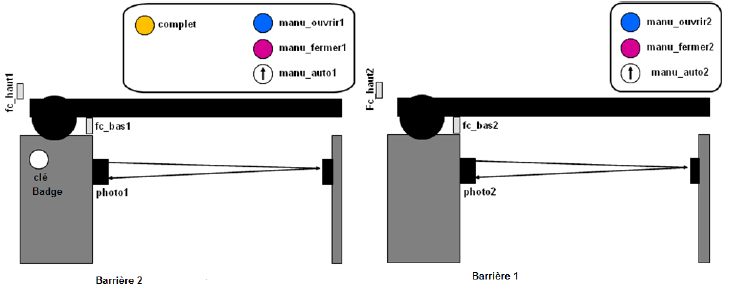
\includegraphics[width=.8\linewidth]{images/schemaSysteme}
	\caption{Partie opérative du système de tri de pièce}
	\label{fig:schemaPartieOperative}
\end{figure}
Ce TP traite d'un système d'accès d'un parking composé de deux barrières : une à l'entrée et une à la sortie (Figure~\ref{fig:schemaPartieOperative}). Ce système est piloté par un automate programmable MODICON de la marque SCHNEIDER. On fera, dans un premier temps, un test des capteurs et des actionneurs.
On prendra en main, à cette occasion, l’outil de développement \textbf{EcoStruxure} de \textit{Schneider Electric} pour l’automate. On écrira pour finir une application sous forme d’un GRAFCET, que l’on testera.

\section{Partie opérative}
\subsection{Description}
Le système est constitué de 2 barrières de parking, l’une pour l’entrée, l’autre pour la sortie. Les deux barrières comportent des détecteurs de présence de véhicule ainsi que les capteurs fin de courses des bras. La barrière d'entrée possède un interrupteur à clef pour réserver l'accès au parking (Figure~\ref{fig:schemaPartieOperative}).

Cette partie opérative est composée de :
\begin{itemize}
	\item d’un pupitre de commande constitué d’’un commutateur 2 positions « manu » et « auto ». Dans la position
	« manuelle », un utilisateur peut monter ou descendre la barrière manuellement via les boutons
	« manu\_ouvrir » et « manu\_fermer ». Dans la position « automatique », le déplacement de la barrière est
	contrôlé par un automate programmable.
	\item d’un bouton d’arrêt d’urgence qui arrête le mouvement de la barrière, qu’elle soit en phase de montée ou de
	descente. Ceci est prioritaire sur la commande par l’automate.
	\item d’un capteur photoélectrique « photo » permettant de détecter la présence d’un véhicule.
 	\item de deux capteurs de fin de course « fc\_bas » et « fc\_haut » indiquant si la barrière est en position haute ou
	basse.
	De plus la barrière d’entrée est équipée d’un interrupteur à clé simulant un système d’accès réservé, ainsi que
	de deux voyants.
	La mise en rotation du moteur des barrières se fait grâce à deux signaux de commande « ouvrir\_barriere» et
	« fermer\_barriere ».

\end{itemize}

La liste des différents capteurs et actionneurs ainsi que leur variable assocée est données dans le Tableau~\ref{tab:capteursActionneurs}.

\begin{table}[ht]
\centering
	\begin{tabular}{|ll || ll|}
	\hline
		\multicolumn{2}{|c||}{Capteurs} 				    & \multicolumn{2}{c|}{Actionneurs}                        \\
		Type                                        & Signal associé & Type                     & Signal associé    \\\hline
		\multirow{4}{*}{Capteurs fin de course}     & fc\_bas1       & \multirow{2}{*}{Moteurs} & FERMER\_BARRIERE1 \\
		                                            & fc\_haut1      &                          & OUVRIR\_BARRIERE1 \\
		                                            & fc\_bas2       &                          & FERMER\_BARRIERE2 \\
																						    & fc\_haut2		   &                          & OUVRIR\_BARRIERE2 \\\hline
  	interrupteur à clef											    & clef					 &                          & VTR               \\\hline
		\multirow{3}{*}{Capteurs presence véhicule} & photo1         &                          &                   \\
		                                            & photo2         &                          &                   \\\hline
	\end{tabular}
	\caption{Liste des capteurs et actionneurs}
	\label{tab:capteursActionneurs}
\end{table}

\section{Partie commande (API)}
La partie commande est assurée par un automate \textit{MODICON} du constructeur \textit{Schneider}. Il dispose d'un module d'entrée TOR et d'un module de sortie TOR.

\UPSTIrappel{\begin{itemize}
	\item Les \textbf{capteurs} de la partie opérative sont reliées aux \textbf{entrées} de l'automate.
	\item Les \textbf{actionneurs} de la partie opérative sont reliées aux \textbf{sorties} de l'automate.
\end{itemize}
}
\subsection{Table d'entrée-sortie de l'automate}
Afin de gagner du temps lors du TP, nous fournissons un projet configuré à l'avance. La table des entrées-sorties est incluse à ce projet (Figure~\ref{fig:entreesSorties})
\begin{figure}[h]
	\centering
	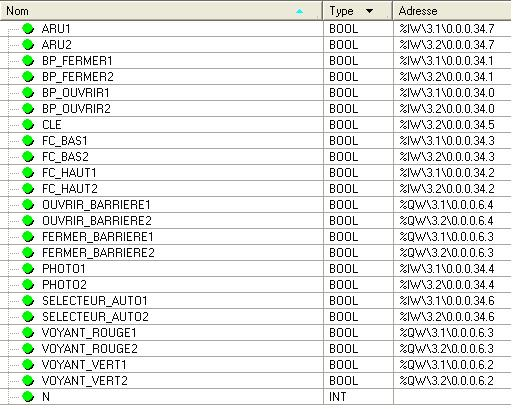
\includegraphics[width=.9\textwidth]{images/listeES}
	\caption{Table des entrées et sorties au sein du projet}
	\label{fig:entreesSorties}
\end{figure}
\pagebreak
\section{Travail demandé}
\subsection{Mise en place informatique}
\begin{UPSTIactivite}[3][Structure du répertoire]
	Dans votre dossier personnel,
	\begin{enumerate}
		\item Créer un dossier intitulé TP03-\nomTP (ou TP04-\nomTP)
		\item Dans ce dossier, créer un dossier \textit{compte-rendu}
		\begin{itemize}
			\item Il contiendra les images, données et le compte-rendu en lui-même
		\end{itemize}
		\item Créer un dossier \textit{projetEcostruxure}
		\item Y copier le contenu du dossier \textit{\nomTP} fourni sur \textit{Commun/Automatisme\_et\_distribution}

	Une fois votre dossier configuré, nous allons compiler et envoyer le projet sur l'automate pour vérifier que la communication entre le PC et l'automate est fonctionnelle.

		\item Ouvrir le projet à l'aide du logiciel \textit{EcoStruxure}
		\item Mettre l'automate sous tension puis compiler et transférer le programme.
		\item Lancer le programme sur l'automate (\textbf{Exécuter})
	\end{enumerate}
\end{UPSTIactivite}

\subsection{Consignes et conseils pour la rédaction du compte-rendu}
Vous rédigerez un compte-rendu détaillé des manipulations effectuées celui du TP 3 servira d'entraînement et comptera avec un coefficient moins important que celui du TP4.

\UPSTIremarque{
Le compte-rendu évalue votre capacité à \textbf{expliquer et synthétiser} votre démarche et les manipulations effectuées.
Les manipulations en elle-même sont observées durant la séance par l'enseignant.}

Vous pourrez donc insérer des captures d'écrans, photos et tout schéma pouvant aider à la compréhension de votre propos.
Un bon compte-rendu est un compte-rendu \textbf{lisible et entièrement compréhensible} par une personne n'ayant pas participé au TP et ayant un niveau de connaissance similaire au vôtre.

\subsection{Prise en main et vérification du fonctionnement du système}
La première chose à vérifier avant d'entreprendre la programmation d'un automate est de vérifier le bon fonctionnement des entrées et sorties de l'automate.
\begin{UPSTIactivite}[][Test des capteurs]
	Avec l'automate sous tension, vérifier \textbf{un à un} le bon fonctionnement de \textbf{tous les capteurs} en vérifiant que la LED correspondante sur le module d'entrées s'allume ainsi que le changement d'état dans la table d'animation du projet.

	Si un capteur ne fonctionne pas ou que son état ne varie pas dans la table d'animation, chercher alors la cause de ce disfonctionnement.
\end{UPSTIactivite}
\UPSTIboiteGenerique{Aide à la rédaction}{\bcplume}{
A titre d'exemple, pour la présentation des tests des capteurs dans votre compte-rendu, vous pouvez expliquer la démarche générale puis insérer une capture d'écran du test d'un des capteurs avec l'explication associée. Il n'est pas alors nécessaire de faire une capture pour chaque capteur.

Précisez également s'il s'agit d'une structure locale ou déportée et décrivez tout disfonctionnement rencontré et comment il a été corrigé.}

\begin{UPSTIactivite}[][Test des actionneurs]
Pour tester les actionneurs, il est nécessaire de commander les sorties de l’automate.

Dans la table d'animation, cliquer sur \textit{Modifications} afin d'activer la commande des sorties.

Vérifier \textbf{un à un} le bon fonctionnement de \textbf{tous les actionneurs} en vérifiant que la LED correspondante sur le module de sortie s'allume et que l'actionneur s'active.
\end{UPSTIactivite}


\subsection{Programmation de l'automate}
\subsubsection{Controles d'accès au parking}
On propose le cahier des charges suivant :
\UPSTIboiteGenerique{Cahier des charges 1 : Commande de la barrière d'entrée}{\bcoutil}{
\begin{itemize}
	\item En présence d'une voiture et de l'activation de l'interrupteur à clef, la barrière s'ouvre
	\item En l'absence de la clef et d'une voiture, elle se referme
	\item Si la voiture réapparait durant la fermeture, la barrière remonte
\end{itemize}}

\begin{UPSTIactivite}[][Implémentation du Cahier des charges 1]
	\label{act:barriereEntree}
	\begin{enumerate}
		\item Dessiner, sur papier ou à l'aide d'un logiciel adapté, le GRAFCET à implémenter
		\item Créer une section dans le projet et implémenter la structure du GRAFCET
		\item Ajouter un commentaire à côté de chage action pour décrire les actions voulues
		\item Implémenter les transitions (penser à créer des sections transitions au besoin, donner des noms \textbf{compréhensibles})
		\item Ajouter et implémenter une section transitions (LADDER ou ST) pour l'activation des actionneurs
	\end{enumerate}
\end{UPSTIactivite}
\UPSTIboiteGenerique{Aide à la rédaction}{\bcplume}{
	A titre d'exemple, dans votre compte-rendu, vous pouvez insérer le GRAFCET ainsi que la section actionneurs. Vous pouvez également expliquer la démarche pour construire un des réseaux du programme LADDER.
}

\UPSTIboiteGenerique{Cahier des charges 2 : Commande de la barrière de sortie}{\bcoutil}{
\begin{itemize}
	\item En présence d'une voiture, la barrière s'ouvre
	\item En l'absence de la voiture, elle se referme
	\item Si la voiture réapparait durant la fermeture, la barrière remonte
\end{itemize}}

\begin{UPSTIactivite}[][Implémentation du Cahier des charges 2]
	Dans une \textbf{nouvelle section} s'ajoutant à la précédente, suivre la même démarche que pour l'activité précédente \ref{act:barriereEntree} pour le cahier des charges 2.

	Les actionneurs peuvent être implémentés dans la même section que pour la barrière d'entrée.
\end{UPSTIactivite}

\begin{UPSTIactivite}[][Initialisation]
	Modifier les GRAFCET des barrières pour le celles-ci se ferment à la mise sous tension. Le comportement normal n'apparaitra alors qu'après que les barrières soient fermées.
\end{UPSTIactivite}

\UPSTIpresenceProf[Faire vérifier le bon fonctionnement]{S'il nest pas disponible, sauvegarder cette version et continuer le TP en attendant.}

\subsubsection{Comptage des véhicule}
\UPSTIboiteGenerique{Cahier des charges 3 : Comptage des véhicule dans le parking}{\bcoutil}{
\begin{itemize}
	\item Les cahiers des charges précédents sont toujours vérifiés
	\item L'automate compte le nombre de véhicules dans le parking
	\item Lorsqu'il y a 3 voitures dans le parking, il est complet
	\begin{itemize}
		\item Un voyant s'allume
		\item Aucun véhicule ne peut entrer dans le parking tant qu'il est complet
	\end{itemize}
\end{itemize}}

\begin{UPSTIactivite}[][Comptage de voitures]
	Afin de réaliser ce cahier des charges, il est conseillé de procéder par étape :
	\begin{enumerate}
		\item Implémenter et tester le comptage de véhicules à l'entrée
		\item Implémenter et tester le décomptage de véhicules à la sortie
		\item
	\end{enumerate}
\end{UPSTIactivite}
\UPSTIboiteGenerique{Aide à la rédaction}{\bcplume}{
	Il serait judicieux de fournir et d'expliquer les modifications apportées aux programmes
}

\begin{UPSTIactivite}[][Alarme]
	Ajouter une alarme si un véhicule est présent devant la barrière d'entrée pendant plus de \SI{7}{s} sans clef.
\end{UPSTIactivite}


\end{document}
